\chapter{Visualisierung}
\label{chp:visualization}

Die Repräsentation von Objekten aus der realen Welt wird mittels Abstraktion und Filterung der essenziellen Merkmale deutlich sparsamer in Bezug auf Datenspeicherung. Die Visualisierung dieser abstrahierten Daten ist definiert als eine ansprechende Darstellung, um eine benutzerfreundliche Interaktion zu ermöglichen. Im Kontext der Effizienz ist die Aufgabe der Visualisierung eine nahtlose Verbindung zwischen der Datenspeicherung und dem Endbenutzer mit einer hohen Performance herzustellen. \cite{modellierung2005glinz,pfefferer1996objektzentrierte}

In diesem Kapitel werden zuerst Eigenschaften der Benutzeroberfläche diskutiert, welche zu einer intuitiven Benutzererfahrung beitragen. Außerdem wird erläutert, von welcher Relevanz Interaktivität und Performance beim Implementieren einer Weboberfläche sind. Des Weiteren werden die unterschiedlichen Arten von Visualisierungsmethoden, zuerst bei einfachen und anschließend bei äußerst komplexen Daten, aufgelistet und erklärt.

\section{Benutzerfreundlichkeit und Performance}

Die Wirksamkeit einer Anwedung hängt nicht nur von deren Benutzerfreundlichkeit, sondern auch von deren Performance ab. Benutzerfreundlichkeit (auch \emph{Usability}) ist die Leichtigkeit, mit den Daten interagieren zu können, und orientiert sich im Idealfall an den Denkweisen des Benutzers. Die Effektivität einer Applikation wird demnach stark von ihrer intuitiven Benutzerbarkeit beeinflusst. \cite{richter1997usability,krug2018think}

Diese Sektion befasst sich mit den drei Begriffen Intuitivität, Interaktivität und Performance im Kontext des \emph{UI-Designs}.

\subsection{Intuitivität}

Benutzer manifestieren die Erwartung, Applikationen ohne Konsultation von Gebrauchsanweisungen und Handbüchern bedienen zu können. Diese Eigenschaft einer Anwendung nennt sich Intuitivität und ist ein Grundsatz moderner Programmsysteme. Intuitivität minimiert die Lernmenge initiativ erheblich. \cite{mardita2017intuitive}

Als Beispiel nehme ich nun die Filterung von Daten her. Benutzer wollen mithilfe der Filterung schneller an die Daten kommen. Aus diesem Grund sollte die Filterung nicht unnötig kompliziert sein, sodass Benutzer zuerst die Filterungsmöglichkeiten verstehen müssen, um diese richtig anwenden zu können. Als Designer dieser Filter muss man sich deswegen einige Fragen stellen: \cite{filter2023vassilatos}

\begin{itemize}
    \item Welche \textbf{Datentypen} sind in meinen Daten enthalten? Boolische Werte können viel intuitiver mittels Ein-Aus-Schalter, als mit Checkboxen, gefiltert werden. 
    \item Welche Daten wird der Benutzer am \textbf{häufigsten filtern}? Der Status eines Paketes ist interessanter als der aktuelle Standort.
    \item Wo soll ich die Filtermöglichkeiten \textbf{platzieren}? Je nachdem, ob die Filter seitlich oder direkt bei den Datenkomponenten angezeigt werden, kann man den Platz unterschiedlich nutzen und unterbewusst verdeutlichen, zu welchen Komponenten die Filter eigentlich gehören.
    \item Zu welchen \textbf{Zeitpunkt}en sollen die Daten neu geladen werden? Während sich für langsame Webseiten ein \wordindoublequotes{Anwenden}-Button über alle Filtermöglichkeiten eignet, können einfachere Filter direkt angewandt werden.
\end{itemize}

Es gibt natürlich noch weitere \wordindoublequotes{best-practice} Tipps, wie zum Beispiel bestimmte Voreinstellungen, welcher der Benutzer öfters brauchen kann. Wie die Filterung schlussendlich gestaltet wird, hängt ganz von den Daten ab. \cite{filter2023vassilatos}

Ein weiterer wichtiger Bestandteil einer barrierefreien Benutzeroberfläche sind \emph{Icons}, da diese Informationen visuell vermitteln und nicht an eine bestimmte Sprache gebunden sind. Somit müssen Benutzer die Systemsprache nicht zwingen verstehen, um eine Anwendung zu bedienen. Dies ist besonders bei Anwendungen für ein internationales Publikum von großer Bedeutung. Eine hohe Priorität hat deswegen die überlegte Auswahl eines verständlichen Iconsets. \cite{icons2024hahn}

Ein weit verbreiteter Mythos des Navigationsdesigns ist die \wordindoublequotes{Three-Click Rule}. Die Grundrichtlinie dieser Regel beschränkt die Anzahl an Klicks oder Eingaben jeglicher Art auf drei, um zu jedem Bereich im Programmsystem zu gelangen. Jedoch stellte sich bei detaillierteren Untersuchungen heraus, dass die Anzahl von Klicks alleine weder Einfluss auf die Benutzerzufriedenheit noch die Erfolgsrate der Applikation hat. Kritik äußert sich demnach aufgrund der Vernachlässigung der kontextuellen Komplexität und individuellen Benutzerziele. \cite{laubheimer2019myth,wright2010myth}

Als nächstes wird die Interaktivität einer Webseite besprochen und welche Auswirkungen diese auf die Benutzererfahrung hat.

\subsection{Interaktivität}

Interaktivität beschreibt eine Eigenschaft eines Inhalts, den Benutzer dazu zu verleiten, sich mit dem Inhalt auseinander zu setzen. Auch wenn das ein wenig geschwollen klingt, trifft diese Beschreibung die Grundidee von Interaktivität recht gut. Der Benutzer ist nicht einfach ein Betrachter des Inhaltes, sondern viel mehr Teil des Prozesses. Es kann sich bei Interaktivität um einfache Hyperlinks, online Quizze, Videos oder sogar Virtual Reality handeln. Wie eine Studie zeigt, bevorzugen 45 Prozent der Menschen interaktive Inhalte. Dies ist unter anderem auch ein Grund, warum Menschen gerne Videospiele spielen, da die Interaktivität dort besonders hoch ist. \cite{interactive2020Ediger}

\begin{quote}
    \say{Interaktivität ist das Potenzial eines technischen Einzelmediums oder einer Kommunikationssituation, das interaktive Kommunikation begünstigt, also den Prozess der Interaktion.} - \textit{Christoph Neuberger}
    \cite{neuberger2007interaktivitat}
\end{quote}

Die Integration effektiver Filter- und Suchfunktionen in Datenvisualisierungssystemen spielt eine Schlüsselrolle bei der Optimierung der Benutzererfahrung und der gezielten Extraktion relevanter Informationen. Untersuchungen haben deutlich gemacht, dass die gezielte Implementierung von sorgfältig gestalteten Filteroptionen in Datenvisualisierungssystemen die Nutzerbefähigung zur gezielten Suche nach spezifischen Datenpunkten oder Mustern in hohem Maße verbessert. Dies resultiert wiederum in einer signifikanten Steigerung der Effizienz innerhalb des Datenmanagements. \cite{morville2010search}

Eine wichtige Komponente ist die Anpassungsfähigkeit der Filter, um unterschiedlichen Anforderungen gerecht zu werden. Die Möglichkeit, Filterkriterien zu kombinieren oder anpassbare Parameter festzulegen, ermöglicht eine feinere Steuerung und eine präzisere Datenauswahl. Dies trägt dazu bei, dass Benutzer ihre Anfragen flexibel an die Komplexität des Datensatzes anpassen können. \cite{shneiderman1996eyes}

Forschungen von Shneiderman et al. betonen die Bedeutung von \emph{Dynamic Queries}, einer Technik, bei der Benutzer unmittelbares Feedback zu ihren Filteranfragen erhalten. Diese Echtzeit-Rückmeldung erleichtert Benutzern eine explorative Analyse. Des Weiteren haben Studien gezeigt, dass die Integration von Vorschlägen während der Eingabe (Autovervollständigung) und die Verwendung von Synonymen die Benutzerfreundlichkeit der Suchfunktionen verbessern. Diese Erkenntnisse verdeutlichen die Relevanz einer kontinuierlichen Forschung und Weiterentwicklung von Filter- und Suchmechanismen, um den sich ständig ändernden Anforderungen der Benutzer gerecht zu werden. \cite{morville2010search,ahlberg1992dynamic}

\subsection{Performance}

Die Effizienz von Webanwendungen spielt eine entscheidende Rolle in der Gestaltung einer ansprechenden Benutzererfahrung. Zahlreiche Studien haben sich mit der Leistungsoptimierung von Webseiten befasst und zeigen, dass eine schnellere Ladezeit einen unmittelbaren Einfluss auf die Zufriedenheit und Interaktion der Nutzer hat. In diesem Zusammenhang präsentiert eine umfassende Untersuchung von Souders, wie die Minimierung von HTTP-Anfragen, das effiziente \emph{Caching} von Ressourcen und die Reduzierung von DNS-Lookups als kritische Elemente für die Optimierung der Webseitenleistung gelten. \cite{souders2008high}

Besonders relevant für die Verbesserung der Benutzerfreundlichkeit sind Optimierungstechniken wie \emph{Lazy Loading} und \emph{Indexing}. Lazy Loading ermöglicht es, Ressourcen nur dann zu laden, wenn sie vom Nutzer angefordert werden, was die Interaktivität beschleunigen kann. In Bezug darauf zeigen Forschungen auf, dass eine effiziente Indexierung von Inhalten die Navigation und den Zugriff auf relevante Informationen für die Nutzer erheblich verbessert. \cite{sharma2020usability,hogan2014speed,jorgensen1996index,barnum2004index}

Aktuelle Studien von Hogan zeigen, dass die Optimierung von HTML, CSS und Bilddateien sowie die Verbesserung der Performance unter Berücksichtigung der steigenden Prozentwerte der mobilen Internetnutzung von besonders hoher Wichtigkeit sind. Diese Erkenntnisse betonen die Bedeutung von Leistungsoptimierungstechniken in der Webentwicklung und vor allem auch in der mobilen Appentwicklung und verdeutlichen, wie diese direkte Auswirkungen auf die Benutzerfreundlichkeit haben können. Die ganzheitliche Berücksichtigung von Aspekten wie Minimierung von HTTP-Anfragen, effizientes Ressourcen-Caching, Lazy Loading und Indexing kann somit als Schlüssel zur Schaffung einer optimalen Nutzererfahrung dienen. \cite{hogan2014speed}
\section{Arten von Datendarstellungen}

Die Visualisierung von hochvernetzten Daten ist heutzutage von zentraler Bedeutung, um die Herausforderungen bei der umfassenden Analyse und Deutung dieser komplexen Datenstrukturen zu bewältigen. Datengefüge solcher Art, die sich beispielsweise in sozialen Netzwerken, biologischen Systemen, Nahrungsketten, Dateisystemen oder sogar in der Struktur der Sprache manifestieren, erfordern spezialisierte Visualisierungstechniken zur Extraktion ihrer inhärenten Muster und Strukturen. \cite{fry2008visualizing}

Bevor die bewährtesten Darstellungen von stark vernetzten Daten erläutert werden, werden noch Visualisierungen von kleineren und einfacheren Datenmengen erklärt.

\subsection{Darstellung von einfachen Daten in Tabellen, Diagrammen und Kennzahlen}

Die Visualisierung von Daten definiert sich als eine grafische Repräsentation, welche korrelierende Daten und logische Relationen nicht nur kommuniziert, sondern auch zu besseren Entscheidungsfähigkeit der Benutzer führt, da diese sachlich unterlegt und begründet sind. Einfache Visualisierungen, wie Balken-, Säulen-, Linien-, Kreis- oder Punktwolkendiagramme, genauso wie Wärmekarten, Tabellen und Kennzahlen in Prozent und anderen Einheiten eignen sich wunderbar für Berichte aus Marketingkampagnen, Leistung eines Vertriebsteams, Produktakzeptanzraten und vor allem für moderne Dashboards. Dashboards geben dem Benutzer einen schnellen Überblick über die verschiedensten aktuellen Daten, damit der Benutzer priorisieren kann, welche Daten näher unter die Lupe genommen werden müssen, um bestmögliche Entscheidungen zu treffen. \cite{2020simplevis}

In Abbildung \ref{fig:einfacheDatenvisualisierung} sehen Sie einige Beispiele dieser einfachen Darstellungsarten aufgezeichnet. 

\begin{figure}
    \centering
    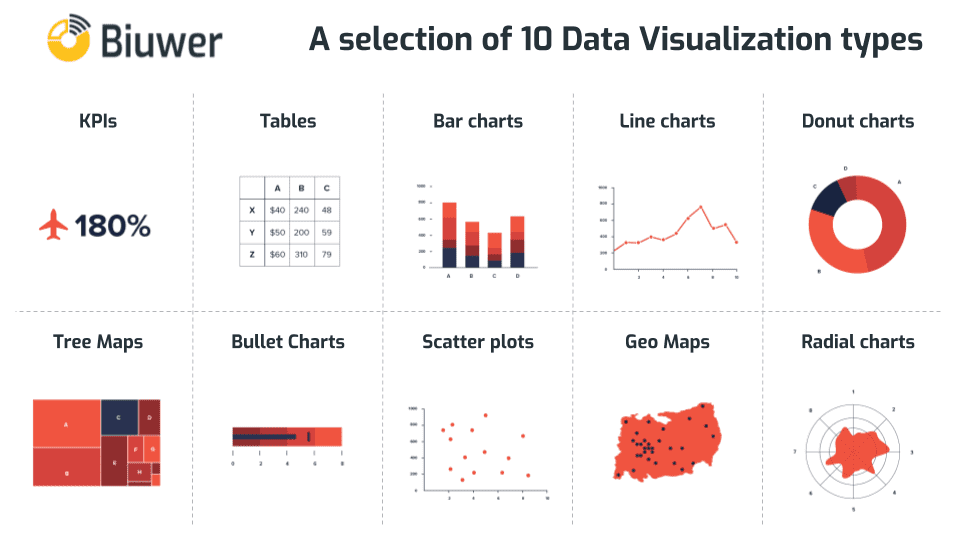
\includegraphics[width=1\textwidth]{content/img/Research/Visualisation/simple_visualisation_methods.png}
    \caption{Einfache Datenvisualisierungen in Form von Werten, Diagrammen, Tabellen und Karten \cite{morales2020picture}}
    \label{fig:einfacheDatenvisualisierung}
\end{figure}
\FloatBarrier

% paar Vor- Nachteile für verschiedene Diagramme

Die Visualisierungen in Abbildung \ref{fig:einfacheDatenvisualisierung} halten sich auch an wichtige Empfehlungen, um eine erfolgreiche Darstellung zu erstellen. Grafiken sollen laut Katy French nämlich eine vollkommene Geschichte erzählen. Dabei wird vor einer Überflut an Daten innerhalb der Visualisierung gewarnt, welche vom wesentlichen Grundgedanken der Darstellung ablenken würden. \cite{frenchsimplevis}

Ein weiterer Tipp bezieht sich auf die Auswahl einer bestimmten primären Farbe, welche mittels Helligkeit und Sättigung mehrere Farbtöne für das Diagramm erzeugt. Zusätzlich ist es immer sinnvoll, Beschriftungen leserlich zu gestalten, die Daten intuitiv zu ordnen und keine Elemente in Darstellungen einzufügen, welche zum Beispiel bei Präsentationen nur dazugesagt werden. \cite{frenchsimplevis}

Beim Designen eines Dashboards sind die Differenzen der verschiedenen Diagramme zu beachten. Denn nicht jedes Diagramm kann von Menschen mit der gleichen Effizienz interpretiert werden und einige Datensätze können in bestimmten Diagrammen nicht gut visualisiert werden. Balkendiagramme stellen Prozentwerte beispielsweise deutlich veranschaulicher dar, als Kreisdiagramme, da letztere die Bogenlänge als Maß für die Proportionalität nehmen. Nur durch richtige Anordnung der Kreissegmente können Benutzer die Daten richtig extrahieren. In Balkendiagrammen werden die Datensätze oft absteigend nach Proportionalität sortiert. \cite{2023diagrammarten}

Auch zwischen Säulen- und Balkendiagrammen gibt es Differenzen. Denn intuitiv befindet sich der Zeitfaktor in jedem Diagramm auf der x-Achse. Deswegen werden Vergleiche über einen gewissen Zeitraum immer mittels Säulendiagrammen dargestellt. Handelt es sich um einen längeren Zeitraum, dessen Gruppierungen die Anzahl 15 überschreiten, wird empfohlen, ein Liniendiagramm stattdessen zu wählen, da sonst zu viele Säulen vorhanden sind. Balkendiagramme eignen sich wiederum besonders für kategoriale Vergleiche, wie zum Beispiel verschiedene Genre bei Büchern und dessen Beliebtheit (Abbildung \ref{fig:GenreBuecherBeliebtheit}). Gruppierte Säulen- beziehungsweise Balkendiagramme sind immer dann zu wählen, wenn pro Zeiteinheit beziehungsweise Kategorie mehrere Datensätze bestehen. Falls diese Datensätze Mengen beschreiben, wie zum Beispiel Anzahl an Frauen und Männern - zusammengerechnet ergibt sich die Anzahl an Personen -, sind gestapelte Säulen- und Balkendiagramme eindeutig zu bevorzugen. In Darstellung \ref{fig:differentCharts} können Sie den Unterschied zwischen gruppierten und gestapelten Säulendiagrammen erkennen. \cite{marktler2020diagrammtypen}

\begin{figure}
    \centering
    \begin{subfigure}{.5\textwidth}
        \centering
        \includegraphics[width=0.9\linewidth]{content/img/Research/Visualisation/gruppiertes_Säulendiagramm.png}
        \caption{gruppiertes Säulendiagramm \cite{groupedChart}}
        \label{fig:groupedChart}
    \end{subfigure}%
    \begin{subfigure}{.5\textwidth}
        \centering
        \includegraphics[width=0.9\linewidth]{content/img/Research/Visualisation/gestapeltes_Säulendiagramm.png}
        \caption{gestapeltes Säulendiagramm \cite{stackedChart}}
        \label{fig:stackedChart}
    \end{subfigure}
    \caption{verschiedene Arten von Säulendiagrammen (auch bei Balkendiagrammen möglich)}
    \label{fig:differentCharts}
\end{figure}
\FloatBarrier

\begin{figure}
    \centering
    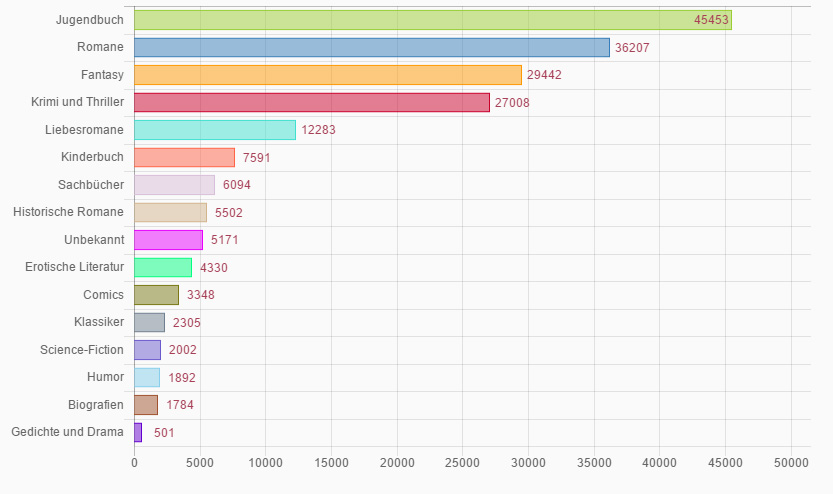
\includegraphics[width=1\textwidth]{content/img/Research/Visualisation/genres.jpg}
    \caption{Beliebtheit der verschiedenen Buchgenre im Jahr 2016 \cite{zeising2016genre}}
    \label{fig:GenreBuecherBeliebtheit}
\end{figure}
\FloatBarrier

Jede Diagrammart hat demnach ihre Daseinsberechtigung und soll auch für den spezifischen Anwendungsfall herangezogen werden. \cite{marktler2020diagrammtypen}

\subsection{Darstellung von komplexen Daten in Graphen, Heatmaps und Diagrammen}

Das Visualisieren von Daten allgemein - unabhängig von der Menge - unterstützt uns wesentlich bei Entscheidungen. Diese Hilfe bei der Findung relevanter Entscheidungen ist einer der essenziellsten Existenzgründe für Darstellungen im Allgemeinen. Die Herausforderung bei der grafischen Aufbereitung von stark vernetzten Daten liegt in der schieren Menge der Daten. Man spricht von \emph{Big Data}. \cite{2020simplevis,lin2023guide}

Pohan Lin erklärt in seinem Artikel die Schwierigkeit, große Datenmengen auf einfachen Bildschirmen intuitiv zu visualisieren, sodass Muster und Zusammenhänge erkannt und demenstprechend auch objektiv sinnvolle Schlüsse aus Daten gezogen werden können. Ebenso erläutert Eberhard Heins in einem Artikel von 2017 die Herausforderungen, welche mit der Visualisierung von Big Data kommen. Mit steigender Anzahl an Knoten und Kanten in einem Graphen wird dieser unübersichtlicher, da Muster in dem \wordindoublequotes{Farbteppich} nicht extrahiert werden können, was die Entscheidungshilfe signifikant reduziert. Ebenso leidet die Orientierung und Leserlichkeit der Darstellung darunter. Nur unter effizienter und übersichtlicher Umsetzung einer Big Data-Darstellung können die Vorteiler der Visualisierung genutzt werden. \cite{lin2023guide,heins2017herausforderungen}

Um ein ungefähres Bild von der schieren Menge an Informationen bei hoch korrelierenden Daten zu bekommen, wird Abbildung \ref{fig:BigData} hier kurz erläutert. Es handelt sich um eine Darstellung des sozialen Netzwerkes LinkedIn. In diesem Graphen hat jeder Konten die Bedeutung einer Person und jede Kante beschreibt eine Art von Beziehung zwischen den beiden anliegenden Personen. Die Extraktion hilfreicher Informationen kann bei Anbetracht dieser Grafik vergessen werden.

\begin{figure}
    \centering
    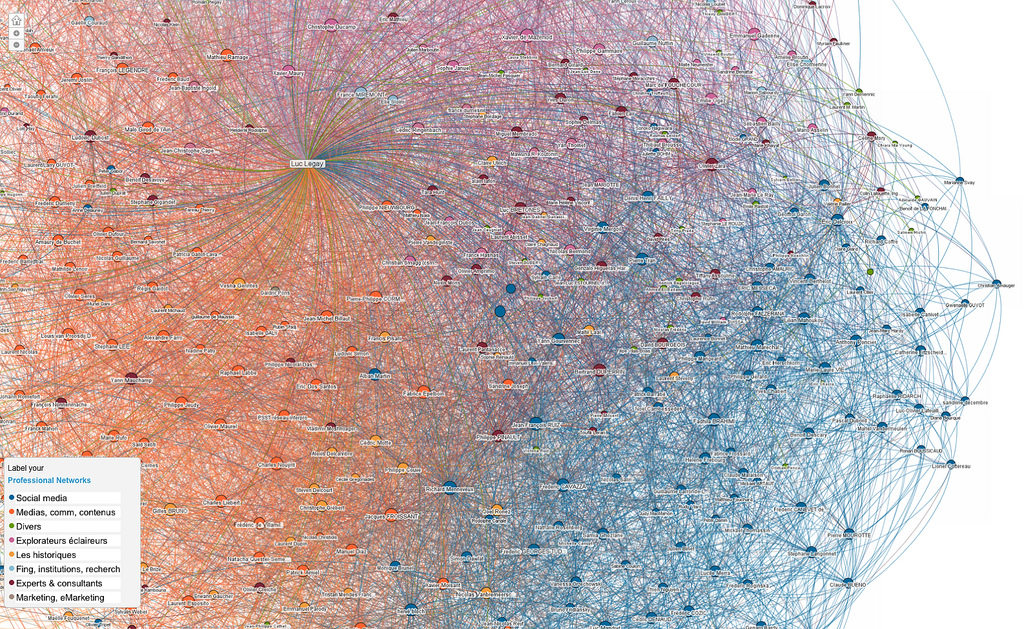
\includegraphics[width=1\textwidth]{content/img/Research/Visualisation/big_data_2.png}
    \caption{Stark vernetzte Daten in einem Graphen (LinkedIn Netzwerk) \cite{bigdata2014image}}
    \label{fig:BigData}
\end{figure}
\FloatBarrier

Die Komplexität eines Graphen kann mittels unterschiedlichen Ansätzen reduziert werden. Logischerweise führt eine Reduktion der Datenmenge automatisch zu einer übersichtlicheren Visualisierung und infolgedessen zu einer besseren Orientierung und Leserlichkeit beziehungsweise Erkennbarkeit. Jedoch kommt die Reduktion mit dem großen Nachteil des Informationsverlustes. Ein weiterer Ansatz definiert aggregierte Visualisierungstechniken als Zusammenfassung gewisser Informationen (\emph{Clustering}). Im Folgenden werden verschiedene Darstellungsmethoden im Detail analysiert. \cite{heins2017herausforderungen}

\subsubsection{Vereinfachung der komplexen Daten mittels Clustering}

Graph-Clustering ist eine Methode zur Vereinfachung eines komplexen Graphen, indem Gruppierungen, Muster, Zusammenhänge oder Strukturen mittels Algorithmen extrahiert werden. Diese neuen Daten sind entscheidend für Datenwissenschaftler. Denn aus den Erkenntnissen dieser können fundierte Entscheidungen in verschiedenen Bereichen, wie zum Beispiel Marketing, Bioinformatik oder auch die Entdeckung von Fehlern oder Sicherheitslücken innerhalb eines Netzwerkes, getroffen werden. \cite{pusic2023clustering}

Die Algorithmen hinter Graph-Clustering sind unterstützt von maschinellem Lernen. Die künstliche Intelligenz versucht hierbei Gemeinsamkeiten der einzelnen Nodes innerhalb des Graphes zu finden. Diese Ähnlichkeiten können entweder direkte Eigenschaften der Knoten sein oder Berechnungen aufgrund der Konnektivität zwischen den Knoten im Graphen. In Abbildung \ref{fig:GraphClusteringAlgorithm} kann auf der rechten Seite die Gruppierung der Knoten des Ausgangsgraphen (links) mittels farblichen Markierungen festgestellt werden. \cite{pusic2023clustering}

\begin{figure}
    \centering
    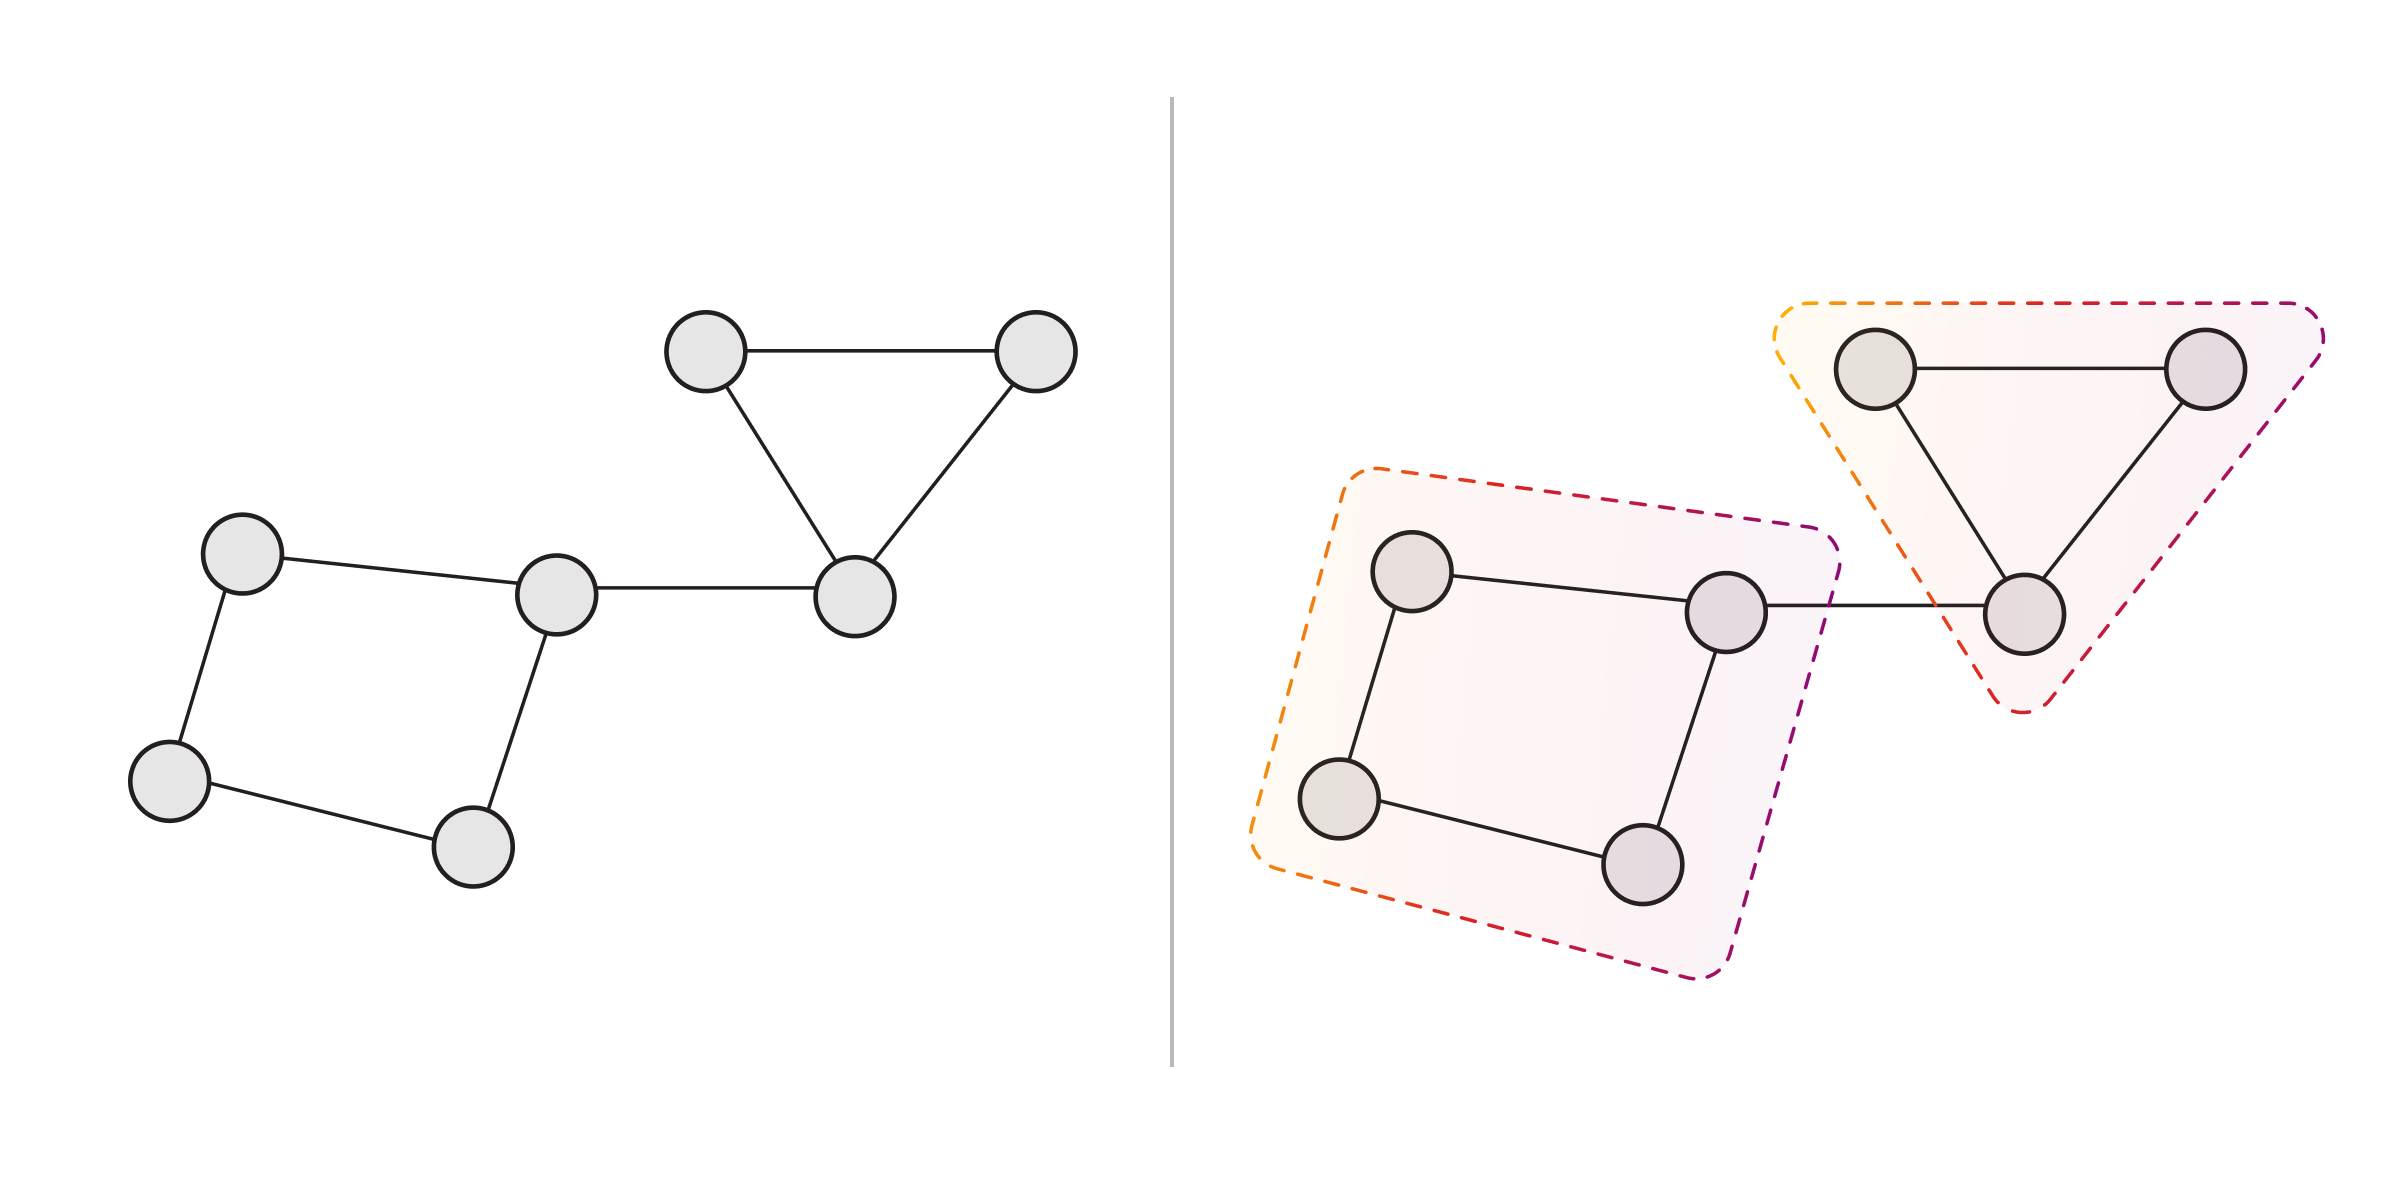
\includegraphics[width=1\textwidth]{content/img/Research/Visualisation/graph_clustering_algorithm.png}
    \caption{Clustering eines Graphen \cite{pusic2023clustering}}
    \label{fig:GraphClusteringAlgorithm}
\end{figure}
\FloatBarrier

Das Clustering eines Graphen kann auch nur auf irrelevante Daten angewandt werden, welche jedoch gruppiert in der Visualisierung beibehalten werden sollen. Beispielsweise können aktuelle Daten in der Mitte möglichst detailliert aufbereitet sein, während Daten aus vergangenen und demnach veralteten Jahre rundherum aggregiert dargestellt sind. \cite{heins2017herausforderungen}

\subsubsection{Vereinfachung der verknüpften Daten mittels farblichen Abstufungen}

Solange die Zugänglichkeit einer Grafik auch für Menschen mit Farbsehschwächen gegeben ist, sind Farben ein wunderbarer Weg, um verschiedene Daten in Diagrammen oder auch Grids zu visualisieren. Sogenannte \emph{Heatmaps} eignen sich besonders gut, um eine große Datenmenge geordnet und gruppiert darzustellen. Dabei werden die Daten in einem Diagramm mit zwei Achsen farblich auf Rechtecken dargestellt, wobei die Farbe Auskunft über die Intensität in der jeweiligen Zeile und Spalte gibt. Empfohlen wird eine Verwendung einer Legende, um die Bedeutung der Farben in der Heatmap zu erklären. \cite{yiheatmap,cinar2023heatmap,kassamara2020heatmap}

Beispielsweise können Sie aus der Abbildung \ref{fig:HeatmapGitHub} deutlich ablesen, dass der Benutzer fast ausschließlich an Wochentagen arbeitet. Samstage und Sonntage sind nämlich in den meisten Fällen grau, was laut Legende bedeutet, dass keine Contributions von diesem Benutzer an diesen Tagen gemacht worden sind. Und genau solche Informationen sind in vielen anderen Bereichen entscheidend für Datenwissenschaftler.

\begin{figure}
    \centering
    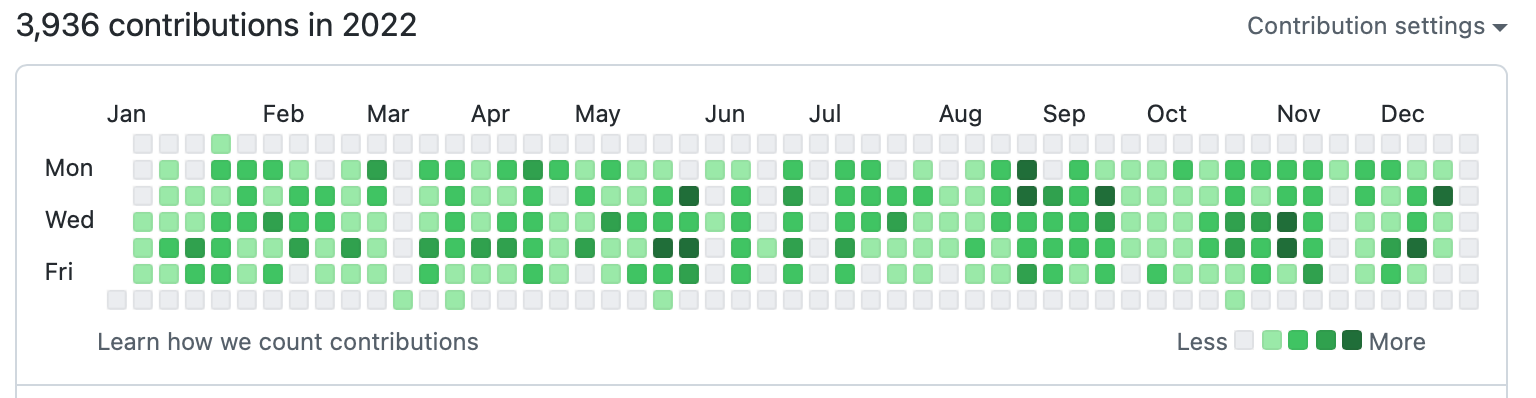
\includegraphics[width=1\textwidth]{content/img/Research/Visualisation/heatmap.png}
    \caption{Heatmap der Beiträge eines GitHub Benutzers im Jahr 2022 \cite{yiheatmap}}
    \label{fig:HeatmapGitHub}
\end{figure}
\FloatBarrier

\subsubsection{Vereinfachung der vernetzten Daten mittels Interaktivität}

Die Visualisierung von Graphen inkludiert meistens eine Zoom- und Filterfunktionalität. Neben diesen Orientierungshilfen gibt es auch die Möglichkeit, Daten in Diagrammen und Graphen mittels Lupentechniken zu vereinfachen. Dabei werden gewisse Daten mittels Verzerrungen hervorgehoben und die restlichen Daten nur verkleinert am Rande angezeigt. Das explorative Verhalten der Visualisierung wird umso mehr verbessert, wenn die Lupenfunktionalität mit dem Benutzer interagiert. Eine besonders intuitive Interaktionsmöglichkeit ist die Lupenverfolgung des Mauszeigers. In anderen Worten kann der Benutzer die Position der Lupe in der Grafik mittels Maus direkt beeinflussen. \cite{bostock2012fisheye}

In Abbildung \ref{fig:LupentechnikGridFisheye} kann das Prinzip der Lupe auf einem Grid gut erkannt werden. Die Verzerrungsmethode heißt hierbei \emph{Fisheye}.

\begin{figure}
    \centering
    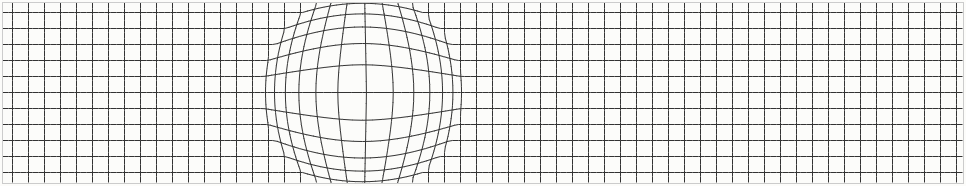
\includegraphics[width=1\textwidth]{content/img/Research/Visualisation/distortion_fisheye.png}
    \caption{Demonstration der Lupentechnik Fisheye auf einem Grid \cite{bostock2012fisheye}}
    \label{fig:LupentechnikGridFisheye}
\end{figure}
\FloatBarrier

Auch, wenn ein statisches Bild den Effekt eines Fischauges in einem Graphen nicht perfekt veranschaulichen kann, sehen Sie in Abbildung \ref{fig:FisheyeGraph} einen Graphen, dessen Knotenpunkt \wordindoublequotes{Brujon} momentan mittels Lupe analysiert wird.

\begin{figure}
    \centering
    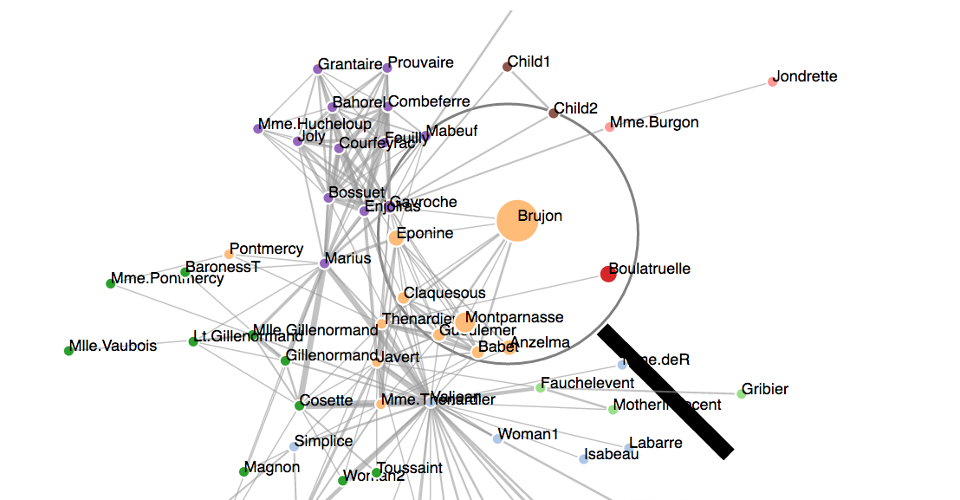
\includegraphics[width=1\textwidth]{content/img/Research/Visualisation/fisheye_graph.png}
    \caption{Demonstration des Fischauges in einem Graphen \cite{githubgistFisheye}}
    \label{fig:FisheyeGraph}
\end{figure}
\FloatBarrier

Die Lupentechnik muss nicht immer mit dem Fisheye-Effekt visualisiert sein. Es gibt zum Beispiel auch die Möglichkeit, eine \emph{kartesische Verzerrung} (Abbildung \ref{fig:LupentechnikGridCartesian}) interaktiv zu verwenden. Dabei werden die Skalierungen der Achsen je nach Mausposition so angepasst, dass es sich so anfühlt, als wäre der Inhalt darunter am nähesten beziehungsweise größten. \cite{bostock2012fisheye}

\begin{figure}
    \centering
    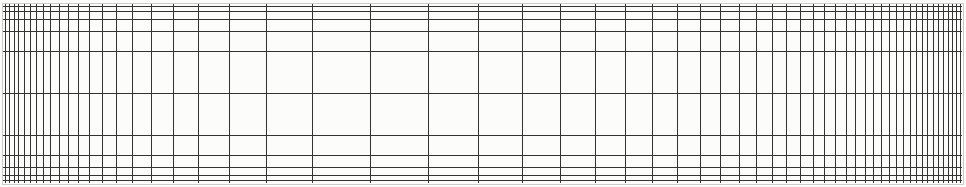
\includegraphics[width=1\textwidth]{content/img/Research/Visualisation/distortion_cartesian.png}
    \caption{Demonstration der kartesischen Verzerrungstechnik auf einem Grid \cite{bostock2012fisheye}}
    \label{fig:LupentechnikGridCartesian}
\end{figure}
\FloatBarrier

\subsubsection{Vereinfachung der vielschichtigen Daten mittels Reduktion}

Die wohl einfachste Methode, stark vernetzte Daten intuitiv und verständlich darzustellen, ist das Entfernen gewisser Datensätze beziehungsweise gewisse Attribute oder Dimensionen von Datensätzen aus der Grafik durch spezifische Filterung der Daten. Dadurch werden nur die wichtigsten Daten angezeigt und der Benutzer kann diese interpretieren und somit vernünftige Entscheidungen daraus schließen. Die Reduktion der Daten hat jedoch den Nachteil, dass einige, eventuell essenzielle Informationen verloren gehen. Bestimmte Zusammenhänge und Strukturen der Daten können nämlich nicht extrahiert werden, wie es jedoch bei anderen Visualisierungsmöglichkeiten (wie zum Beispiel Clustering) der Fall ist. Dieser unvermeidliche Informationsverlust sollte bei der Reduktion minimiert werden, um in Bezug auf Richtigkeit möglichst nahe an den ungefilterten Daten zu bleiben. \cite{heins2017herausforderungen,beilhammer2017interpretation}

\subsubsection{Darstellung der vereinfachten Daten durch Mischformen}

\wordindoublequotes{Best practice}-Visualisierungen vermischen verschiedene Formen der Vereinfachung und erstellen Grafiken, welche die wesentlichsten Informationen kurz und knapp auf den Punkt darstellen. Beispielsweise hat Google in der Dokumentation von Google Maps eine geobasierte Heatmap\footnote{Hierbei wird der Begriff \wordindoublequotes{Heatmap} allgemein verwendet, da diese nicht an ein Raster gebunden ist.} herangezogen, welche in Abbildung \ref{fig:GoogleMapsHeatmap} zu Demonstrationszwecken abgebildet ist.

\begin{figure}
    \centering
    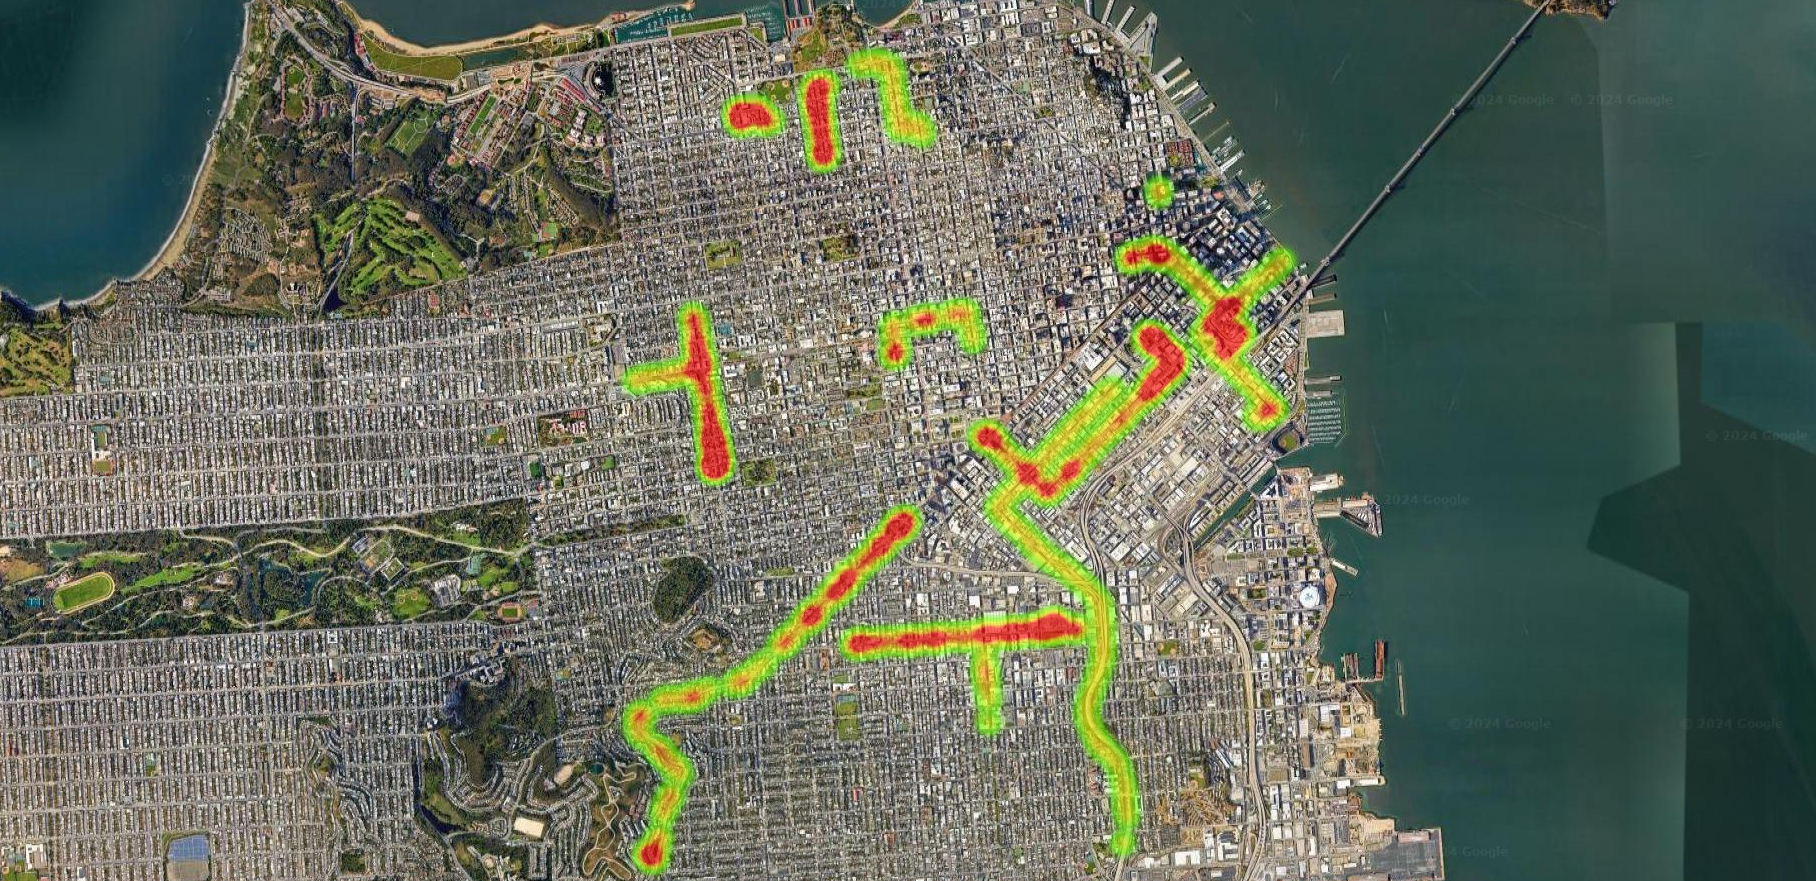
\includegraphics[width=1\textwidth]{content/img/Research/Visualisation/Google_Maps_Heatmap.png}
    \caption{Exemplarische geobasierte Heatmap aus der Google Maps Dokumentation}
    \label{fig:GoogleMapsHeatmap}
\end{figure}
\FloatBarrier
\section{Bibliothek zur visuellen Darstellung insbesondere von Graphen}

Nachdem die theoretischen Visualisierungsmethoden der bestehenden Literatur nun abschließend erläutert worden sind, wird nun eine Bibliothek für die Implementation der Darstellung von Graphen vorgestellt. \emph{Cytoscape} ist eine Bibliothek für auf JavaScript-basierende Applikationen, welche die Erstellung eines Graphen im Frontend wesentlich erleichtert. Häufig wird Cytoscape für biologische Prozesse und Zusammenhänge verwendet, da besonders diese natürlichen wissenschaftlichen Bereiche ähnliche Strukturen wie Graphen aufweisen. Ursprünglich ist Cytoscape auch für genau diese Zwecke an der \wordindoublequotes{University of Toronto} entwickelt und anschließend in \wordindoublequotes{Oxford Bioinformatics} publiziert worden. Die Anwendungsbereiche von Graphenvisualisierungen gehen jedoch weit über den biomolekulare Bereich hinaus. \cite{Cytoscape}

Cytoscape bringt einige Vorteile mit sich. Die Bibliothek ist einfach zu verwenden und verfügt über eine detaillierte Dokumentation. Darüberhinaus gibt es inspirierende Demonstrationen, wie die Bibliothek verwenden werden kann. Diese Beispiele haben bei der Implementierung des Prototypen sehr geholfen. \cite{Cytoscape}

Bemerkenswert an Cytoscape ist auch das Eco-System und die Community, da es nicht nur viele Plugins, sprich Erweiterungen, gibt, sondern auch eine Variation an unterstützen Modulsystemen, darunter \wordindoublequotes{ES modules}, \wordindoublequotes{Node.js} und \wordindoublequotes{AMD/Require.js}. Des Weiteren wird Cytoscape in allen modernen Browsern unterstütz -- eine extrem wichtige Eigenschaft für Frontend-Developer heutzutage. Und genau das sind auch einige der Gründe, warum wir uns für die Verwendung der Bibliothek Cytoscape entschieden haben. \cite{Cytoscape}

Alle Vorteile und Eigenschaften von Cytoscape sind nochmals übersichtlich in Abbildung \ref{fig:CytoscapeArchitektur} dargestellt.

\begin{figure}
    \centering
    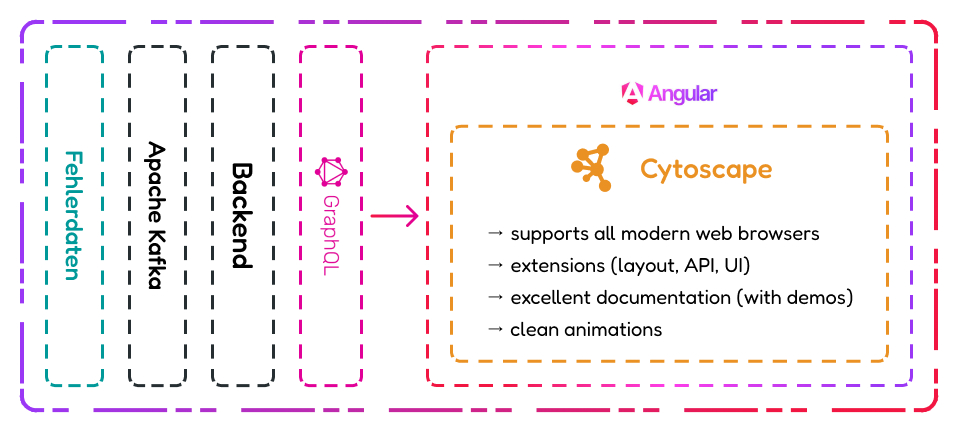
\includegraphics[width=1\textwidth]{content/img/Architecture/Architecture_Cytoscape.jpg}
    \caption{Architektur unseres Prototypen mit Fokus auf die Bibliothek Cytoscape}
    \label{fig:CytoscapeArchitektur}
\end{figure}
\FloatBarrier

Die Darstellungen anderer Grafiken, wie Beispielsweise Diagramme, verwenden jeweils entsprechend passende Bibliotheken. \emph{ng2-charts} eignet sich besonders gut für das Darstellen von Diagrammen in Angular Applikationen und basiert auch der allgemeinen JavaScript Bibliothek für Diagramme, \emph{Chart.js}. \cite{ng2-charts}